\documentclass{article}

\usepackage{corl_2022} % Use this for the initial submission.
%\usepackage[final]{corl_2022} % Uncomment for the camera-ready ``final'' version.
%\usepackage[preprint]{corl_2022} % Uncomment for pre-prints (e.g., arxiv); This is like ``final'', but will remove the CORL footnote.

% ---------------------------------
% Packages
% ---------------------------------
\usepackage{mathtools}
\usepackage{amsfonts}  % for \mathbb
\usepackage{graphics}
\usepackage[pdftex]{graphicx}
\usepackage{wrapfig}
\usepackage{caption}
\usepackage{color}
\usepackage{dsfont}
\usepackage{subcaption}
% \usepackage[symbol]{footmisc}

% % Algorithm.
\usepackage{algorithmicx}
\usepackage[ruled]{algorithm}
\usepackage{algpseudocode}
\usepackage{amssymb}

% ---------------------------------
% Macros
% ---------------------------------

\algnewcommand\algorithmicforeach{\textbf{for each}}
\algdef{S}[FOR]{ForEach}[1]{\algorithmicforeach\ #1\ \algorithmicdo}

% KL Divergence 
\DeclarePairedDelimiterX{\infdivx}[2]{(}{)}{%
  #1\;\delimsize\|\;#2%
}
\newcommand{\infdiv}{\infdivx}
\newcommand{\kld}[2]{\ensuremath{D_{KL}\inf
divx{#1}{#2}}}

% Omit final dot from each def.
\usepackage{expl3}
\ExplSyntaxOn
\newcommand\latinabbrev[1]{
  \peek_meaning:NTF . {% Same as \@ifnextchar
    #1\@}%
  { \peek_catcode:NTF a {% Check whether next char has same catcode as \'a, i.e., is a letter
      #1.\@ }%
    {#1.\@}}}
\ExplSyntaxOff
\def\eg{\latinabbrev{e.g}}
\def\etal{\latinabbrev{et al}}
\def\etc{\latinabbrev{etc}}
\def\ie{\latinabbrev{i.e}}

% Vector.
\let\vec\mathbf

\newcommand{\numconnectors}{35}

% Comments
\providecommand{\kuan}[1]{{\color{blue} [Kuan: #1]}}

\title{Policy Finetuning for Industrial Insertion of Novel Connectors via Domain Generalization}

% The \author macro works with any number of authors. There are two
% commands used to separate the names and addresses of multiple
% authors: \And and \AND.
%
% Using \And between authors leaves it to LaTeX to determine where to
% break the lines. Using \AND forces a line break at that point. So,
% if LaTeX puts 3 of 4 authors names on the first line, and the last
% on the second line, try using \AND instead of \And before the third
% author name.

% NOTE: authors will be visible only in the camera-ready and preprint versions (i.e., when using the option 'final' or 'preprint'). 
% 	For the initial submission the authors will be anonymized.

\author{
  Jane E.~Doe\\
  Department of Electrical Engineering and Computer Sciences\\
  University of California Berkeley 
  United States\\
  \texttt{janedoe@berkeley.edu} \\
  %% examples of more authors
  %% \And
  %% Coauthor \\
  %% Affiliation \\
  %% Address \\
  %% \texttt{email} \\
  %% \AND
  %% Coauthor \\
  %% Affiliation \\
  %% Address \\
  %% \texttt{email} \\
  %% \And
  %% Coauthor \\
  %% Affiliation \\
  %% Address \\
  %% \texttt{email} \\
  %% \And
  %% Coauthor \\
  %% Affiliation \\
  %% Address \\
  %% \texttt{email} \\
}


\begin{document}
\maketitle

%===============================================================================

\begin{abstract}
Industrial insertion tasks, such as inserting connectors in sockets and setting screws, are automated in factories today by robots with specialized control algorithms.
These algorithms rely on precise localization of the connector or socket and carefully managed physical setups, such as assembly lines, to succeed at the task.
If we could instead solve these tasks from visual input without precise localization, many more of these tasks could be successfully automated and also be robust to errors in perception or grasping.
For this to be useful, the method has to generalize to a wide variety of connectors and connector poses.
Offline reinforcement learning followed by online finetuning is a powerful paradigm for learning controllers from data for this kind of generalization: offline RL may not fully generalize zero-shot to novel situations, so online finetuning may be necessary.
In this paper, we present a system towards learning robust vision-only insertion policies that can be fine-tuned with online fine-tuning to a novel, previously unseen connector.
We first collect a diverse dataset of \numconnectors{} different connectors across a variety of backgrounds and two robots.
We then train a policy which can be finetuned with offline RL, using a domain alignment representation learning objective to generalize policies, value functions, and reward models to new connectors.
We show that we can finetune to a novel unseen connector from only vision input without knowledge of the position of the socket or pose estimation of the grasped connector.
%%SL.6.8: Abstract currently doesn't make it clear what the novel contribution of the paper is.

% Offline reinforcement learning followed by online fine-tuning is a powerful paradigm for solving control problems without the need to fully generalize zero-shot to novel situations.
% %%SL.5.25: I think this sentence could be improved, and could use a bit more motivation -- maybe split into two sentences to motivate the parts, otherwise people not already fmailiar with offline RL or finetuning won't really understand *why* this is interesting
% Using this paradigm, we tackle the problem of solving industrial insertion tasks from vision in order to learn robust controllers that can recover from position errors or incorrect grasps.
% %%SL.5.25: This sounds quite nice, if we actually succeed in demonstrating this (but perhaps consider what the "evidence" that this happens would need to look like...)
% We collect data and train a policy with offline reinforcement learning on a wide variety of connectors.
% To finetune from vision, we propose a contrastive domain alignment objective that stabilizes visual features and prevents them from collapsing during finetuning.
% %%SL.5.25: I find it a bit hard to understand the significance of the two sentences above. I think they are trying to describe what the method is, but they don't seem to logically follow from the preceding sentences in the abstract (that is, the first two sentences don't motivate them). Maybe rewrite them in a way that follows more logically?
% We show that we can finetune to a novel unseen connector from only vision input without any state information.
% %%SL.5.25: "state information" is a bit of jargon, it's not really clear what it means in context (a likely misunderstanding is that someone will think it means "without arm position", and it's not clear why that's relevant)
\end{abstract}
%%SL.5.25: I would recommend somewhat rewriting the abstact to make sure that it hits on the main points that are critical to introduce the work: (1) what is the problem; (2) why is it important and difficult; (3) how do we solve this. Right now it's quite clear esp what the answers to (1) and (2) are.
%%AVN.6.1 Rewritten to start with insertion

% Two or three meaningful keywords should be added here
\keywords{Reinforcement Learning, Robotics, Offline RL} 

%==============================================================================


\section{Introduction}

Models that are pre-trained on broad, diverse datasets and can be fine-tuned to specific problems have driven recent progress in vision and NLP~\cite{krizhevsky2012imagenet, devlin2019bert}.
Perhaps the same kind of generalization could be attained in robotics by collecting broad datasets for particular classes of tasks and training general policies from these datasets that can perform these tasks in diverse settings and with varied objects.
However, in robotics, this is a difficult challenge due to hardware, setup, and supervision costs of collecting diverse data.
%%SL.6.8: I don't understand the above sentence -- what is the challenge due to "hardware, setup" and what supervision cost are you talking about? I would suggest just rewriting it, as right now it kind of reads like a "generic" motivation (and one that is somewhat logically inconsistent)
Existing datasets~\cite{ebert2021bridge, dasari2019robonet} are still limited to one or few robots, performing tasks in a few distinct domains with highly correlated background, objects, and tasks within a domain.
%%SL.6.8: kind of implies that a contribution of this paper is to collect a broader dataset, which is not actually the case
Generalizing to a new domain from prior data of few domains is difficult, so in robotics we need more than the paradigm of learning from offline datasets and generalizing zero-shot.
On the other hand, robotics offers a unique opportunity in being able to interact online in the test environment and collect new data.
The online data can provide extra signal for adapting representations to perform well in the new domain.
Instead of expecting perfect zero-shot generalization, if we could learn from offline datasets containing few domains, then fine-tune on a task in a new domain, it would greatly broaden applicability of learning-based robotics.
%%SL.6.8: I would recommend rewriting the above paragraph. I do think it has the right idea, but the sentences do not follow each other in a logical manner. Try to think of the main idea you want to get across and make sure that each sentence builds on the previous one and there is a clear logical progression.

We study this problem in the setting of learning a policy from vision for performing industrial insertion tasks.
This family of assembly tasks, including plugging in connectors into sockets, screwdrivers into screw intrusions, setting screws, and so on, are found in many stages of manufacturing.
%%SL.6.8: Good, but don't overclaim! The paper is not doing "screwdrivers into screw intrusions".
When automated in factories today, these tasks are done by robots with specialized control algorithms that rely on precise localization of the socket location.
% In many instances, humans are required to do these tasks instead because the environment cannot be carefully controlled.
For robots to perform these insertion tasks in industrial and warehouse settings with less human supervision, or in unstructured environments such as homes, they cannot rely on highly accurate state information
%%SL.6.8: I really don't think that most people will think "state information" = socket location. The first few times I read this, I was sure "state information" meant robot state (i.e., joint angles). Maybe use a different terminology?
and must generalize from vision.
%%SL.6.8: The above doesn't really explain the problem. Is the problem to insert one connector? "generalize" to what?
But collecting broad datasets in this domain for visual generalization is a challenge because collecting data for each connector requires significant setup and supervision. 
%%SL.6.8: but isn't collecting such a dataset precisely what this paper does?
% Errors could be introduced in localizing the socket, grasping the connector, and so on, which can make state-based algorithms brittle.
% Instead, if robots had semantic visual understanding of connector-socket insertion tasks and feedback visuomotor control policies to accomplish them, a much broader array of these tasks could be automated.
Among these tasks, there is enough variability to require generalization and adaptation, but also enough internal structural regularity that we expect transfer between different connectors.
How can a robot generalize from vision to test connectors in this setting, utilizing offline reinforcement learning but also active online fine-tuning?
%%SL.6.8: These last two sentences are great! But it would be good for the rest of the paragraph to be improved to lead up to that

The key insight is that we need to learn representations that (1) find common structure between domains while preserving important domain-specific information and (2) can be adapted for new tasks quickly with online data.
%%SL.6.8: The above sentence reads very well!
For finding common structure while preserving important domain-specific information, we propose a split representation that combines domain adversarial neural networks~\cite{ganin2016domainadversarial} for domain invariance and a variational information bottleneck~\cite{alemi2017vib}
%%SL.6.8: not the right citation for VIB!
for controlling the flow of domain-specific information.
% We propose to use an auxiliary contrastive representation learning objective that aligns disparate domains to address this issue.
%%SL.5.25: not quite clear what "disparate domains" refers to here
% To learn low-dimensional representations from large (160x160) image input for sample-efficient RL, we use the standard self-contrastive learning objective with data augmentations.
%%SL.5.25: that doesn't sound like a contribution, it kind of just sounds like we use a thing that already exists
%%AVN.6.2 Rephrased to emphasize the new thing (but agreed it is not super novel)
To align data from diverse domains, we propose to use a self-contrastive learning objective, contrastive domain alignment (CDA),
%%SL.6.8: is this an existing algorithm? if so, cite it; writing wise, maybe add a bit of motivation for why we do this?
with data augmentations additionally treating all observations with positive rewards (i.e., images of successful insertions) as positives.
%%SL.6.8: The above sounds good (if a bit laundry-list), but the stuff below doesn't follow logically from the above. Should these be separate paragraphs? Feels like there is a very sudden jump right here.
To train models to generalize to test connectors, we first collected a large offline dataset with insertion data of \numconnectors~connectors across 2 robots and diverse backgrounds with actions, images, and clean sparse reward labels.
We show that the CDA representation learning objective helps train policies that generalize better from offline training to an unseen connector. 
%%SL.6.8: definitely doesn't belong in the same paragraph -- don't mix together the summary/motivation of the technical method and the results like that
Then, during online finetuning, this auxiliary objective can be used in combination with online RL with a high number of gradient updates per environment step to stabilize and accelerate learning.
For finetuning without state information, we require an accurate reward model that generalizes.
We demonstrate that with the CDA representation, our reward function on a test connector is more accurate.
Then during finetuning, we achieve a higher success rate in X minutes of finetuning using CDA than using alternative domain transfer objectives.
%%SL.6.8: The first half of the above paragraph (about the contrastive thing) reads well, but the stuff afterwards (To train models...) again is a bit incoherent, with sentences not following logically from one another. Probably that should be a separate paragraph, but it likely also needs to be somewhat rewritten to flow more smoothly

% Contributions
We present two major contributions.
First, we propose a novel representation learning method that allows better generalization of policies and reward functions.
This enables fast finetuning of vision-based IQL
%%SL.6.8: first time IQL is mentioned
policies on a new domain. 
%%SL.6.8: nothing in the above sentences talks about offline training on multiple connectors... kind of weird
Second, we present a system based off of this representation learning method to insert robustly from vision without the need of state information,
%%SL.6.8: see above comment about "state information"
both for observations and rewards.
We show that new tasks can be learned within X trials, given our dataset of off-policy data from Y prior tasks of Z trajectories.
This system allows us to finetune IQL to a test connector with significantly higher performance.
Our dataset of robotic insertion of \numconnectors connectors, as well as pretrained features and reward models will be made public at <URL>.

% We face several challenges .
% First, no existing public dataset contains data of diverse insertion tasks with image input.
% %%SL.6.2: I think the bar for presenting a public dataset that people can use is much higher than what this paper is likely to accomplish, so I would not recommend claiming that the release of a public (reusable) dataset is one of the contributions unless you are prepared to put in the work to make it usable and convince the readers of this (which I don't think is entirely realistic in the remaining time). If we're not claiming that, then we shouldn't motivate from this perspective.
% We collected a large offline dataset with insertion data of \numconnectors connectors across 2 robots and diverse backgrounds with actions, images, and clean sparse reward labels.
% %%SL.6.2: Before talking about what we do, we should motivate the approach.
% We use this data for offline RL but release it publicly so it can be used by others for domain adaptation, dynamics understanding of contact-rich tasks, or finetuning to their own insertion problems.
% %%SL.6.2: Good to note we release it, but not so prominently (because you won't be able to convince readers that this is useful)
% Second, we utilize offline RL to learn policies on this data, but it may not generalize zero-shot to all potential insertion tasks.
% %%SL.6.2: This needs to be motivated earlier.
% Instead of relying solely on zero-shot generalization, we can also fine-tune the policy with additional data collected online on the target connector.
% For finetuning, we need an accurate reward function, since we cannot rely on state information for rewards either.
% Finally, since there is a relatively high setup cost of collecting data on individual connectors, the dataset is highly correlated and only contains around \numconnectors visually distinct settings.
% All these learned models - policies, value functions, and rewards, they need to generalize from a small number of individual domains (connectors, robots, and backgrounds) to a new domain.

% What does it take to fine-tune on test environments?
% First, to improve in a test environment we need not only a policy that generalizes but also a reward model. 
% First of all we need an accurate reward model.
% Second, we need algorithms that can train offline and finetune.
% Third, we need generalization of .

% Describe domain adaptation representation learning method

% Contributions

% The success of deep learning
% Deep learning for vision-based robotics
% But its hard to collect robotics in data
% For example, consider industrial insertion
% The idea is best evaluated on a family of tasks where there is enough variability to require generalization and adaptation, but also considerable internal structural regularity so that we have reason to expect things to generalize.
% Consider learning a policy from vision for performing industrial insertion tasks, a frequently encountered problem in manufacturing.
% Few-domain datasets
% Zero-shot generalization is hard
% Instead we can fine-tune

% What does it take to fine-tune?
% First we need rewards
% We need algorithms that can train offline and finetune
% We also need generalization


% \section{Introduction}

% % what is the problem
% Industrial insertion is a frequently encountered problem in manufacturing. This family of assembly tasks, including plugging in connectors into sockets, screwdrivers into screw intrusions, setting screws, and so on, are found in many stages of manufacturing.
% When automated in factories today, these tasks are done by robots with specialized control algorithms which rely on precise state information of the socket location and carefully managed physical setups, such as assembly lines, to succeed at the task.
% In many instances, humans are required to do these tasks instead because the environment cannot be carefully controlled.
% For robots to perform these insertion tasks in industrial and warehouse settings with less human supervision, or in unstructured environments such as homes, they cannot rely on highly accurate state information.
% Errors could be introduced in localizing the socket, grasping the connector, and so on, which can make state-based algorithms brittle.
% Instead, if robots had semantic visual understanding of connector-socket insertion tasks and feedback visuomotor control policies to accomplish them, a much broader array of these tasks could be automated.
% %%SL.6.2: I think the introduction still has the same problem I pointed out before: it is motivated from two seemingly unrelated perspectives, both as an application-centric paper focusing on industrial insertion, and as a study of offline RL. We could discuss how to best motivate it, but I'm not sure if a purely insertion-centric motivation will be that successful, because I think if people look at this alongside other works on industrial insertion, I doubt the method will stand out in terms of how well it works for insertion in particular. But the generality of the approach could be more compelling. Perhaps a motivation that discusses the broader, more general motivation with industrial insertion as an application area would work better? E.g., one way you could motivate this is to talk about how the main idea is best evaluated on a family of tasks where there is enough variability to require generalization and adaptation, but also considerable internal structural regularity so that we have reason to expect things to generalize.

% Reinforcement learning from offline data is a promising approach to learn robust feedback control policies from vision that generalize to new connectors and errors in grasping and socket localization.
% %%SL.6.2: But the method is not just about RL from offline data?
% However, there are many remaining challenges applying RL in this setting.
% First, no existing public dataset contains data of diverse insertion tasks with image input.
% %%SL.6.2: I think the bar for presenting a public dataset that people can use is much higher than what this paper is likely to accomplish, so I would not recommend claiming that the release of a public (reusable) dataset is one of the contributions unless you are prepared to put in the work to make it usable and convince the readers of this (which I don't think is entirely realistic in the remaining time). If we're not claiming that, then we shouldn't motivate from this perspective.
% We collected a large offline dataset with insertion data of \numconnectors connectors across 2 robots and diverse backgrounds with actions, images, and clean sparse reward labels.
% %%SL.6.2: Before talking about what we do, we should motivate the approach.
% We use this data for offline RL but release it publicly so it can be used by others for domain adaptation, dynamics understanding of contact-rich tasks, or finetuning to their own insertion problems.
% %%SL.6.2: Good to note we release it, but not so prominently (because you won't be able to convince readers that this is useful)
% Second, we utilize offline RL to learn policies on this data, but it may not generalize zero-shot to all potential insertion tasks.
% %%SL.6.2: This needs to be motivated earlier.
% Instead of relying solely on zero-shot generalization, we can also fine-tune the policy with additional data collected online on the target connector.
% For finetuning, we need an accurate reward function, since we cannot rely on state information for rewards either.
% Finally, since there is a relatively high setup cost of collecting data on individual connectors, the dataset is highly correlated and only contains around \numconnectors visually distinct settings.
% All these learned models - policies, value functions, and rewards, they need to generalize from a small number of individual domains (connectors, robots, and backgrounds) to a new domain.
% %%SL.6.2: I recommend rewriting this paragraph to motivate the approach, not clutter it with talk about releasing a dataset (the dataset is not going to be useful to anyone but us anyway, so it's hard for readers to see this as a serious contribution), and motivate why we do particular things before stating what they are

% % why is it hard
% % While prior methods have addressed connector insertion from vision, they assume relatively accurate state information with $\pm2\text{mm}$. In contrast, we solve tasks from vision with the connector starting $\pm2\text{cm}$ away from the socket. In this setting, simply doing structured exploration is not enough: vision is required.

% %%SL.6.2: The content of this paragraph doesn't seem to be motivated at all in the preceding discussion
% % main components of our approach
% We propose to use an auxiliary contrastive representation learning objective that aligns disparate domains to address this issue.
% %%SL.5.25: not quite clear what "disparate domains" refers to here
% % To learn low-dimensional representations from large (160x160) image input for sample-efficient RL, we use the standard self-contrastive learning objective with data augmentations.
% %%SL.5.25: that doesn't sound like a contribution, it kind of just sounds like we use a thing that already exists
% %%AVN.6.2 Rephrased to emphasize the new thing (but agreed it is not super novel)
% To align data from diverse domains, we use a self-contrastive learning objective with data augmentations additionally treat all observations with positive rewards (i.e., images of successful insertions) as positives.
% We first show that this representation learning objective helps the reward and policy generalize better to an unseen connector. 
% Then, during online finetuning, this auxiliary objective can be used in combination with online RL with a high number of gradient updates per environment step to stabilize and accelerate learning.

% % Contributions
% We present three key contributions.
% First, we propose a novel representation learning method that allows better generalization of policies and reward functions.
% This enables fast finetuning of vision-based IQL policies on a new domain. 
% %%SL.5.25: this is not a complete sentence! also, you said before it's a standard method, but now it's a novel method?
% Second, we present a system based off of this representation learning method to insert robustly from vision without the need of state information, both for observations and rewards.
% We show that new tasks can be learned within X trials, given our dataset of off-policy data from Y prior tasks of Z trajectories.
% This system allows us to finetune a connector with grasping in the loop {\color{blue}
% (assuming this works.)}.
% % Using this system, we collected high-quality insertion data on Y connectors.
% %%SL.5.25: why is this important?
% %%AVN.6.2. I think the dataset is an important contribution; however it looks like it probably will not be collected in an on-policy way. I added discussion of the dataset above though
% Our third contribution is to release a dataset for robotic insertion connectors, as well as pretrained features and reward models.
% %%SL.6.2: really don't think this will work
% %%SL.5.25: this kind of comes out of nowhere, wasn't mentioned or discussed before; if the dataset is one of the contributions, you would need to actually discuss it in detail and explain how it's useful to people (you could just remark that we release the dataset without claiming that it is one of the contributions, if you don't want to deal with this problem)
% Our dataset will be made public at <URL>.

% \section{Introduction}

% Models that are pre-trained on broad datasets and can be fine-tuned to specific problems, sometimes called ``foundation models''
% %%SL.5.25: Kind of a matter of preference, but I'm not big fan of this (re)branding of pretrained models. I suspect it's easy enough to get people to understand what you mean without it.
% have driven recent progress in vision and NLP.
% For instance, bidirection encoders from transformers (BERT) ~\cite{devlin2019bert} pretrained on large language datasets (100Ms of sentences) is now the standard starting point for fine-tuning to language models on custom language tasks and on custom data of much smaller size (10,000s of sentences).
% This type of pretraining capability enables machine learning to be used to solve more bespoke problems, greatly widening the applicability of ML methods to real-world applications.
% Similarly, robotics applications are often narrow, so the ability to utilize broad prior data but fine-tune on a specific task would be extremely valuable.
% %%SL.5.25 I think this is a great story, but I'm just not sure this story really makes sense for the present paper. We are not really training the system on particularly broad or large datasets compared to other work in robotic learning (and arguably many prior papers have used much larger and much broader datasets), so it might kind of rub people the wrong way to scope the claims around this. Generally, people expect that the claims will follow from the motivation, so if the motivation is that effective generalization can be attained from broad and diverse datasets and large models, people will expect to see the paper make a contribution in demonstrating this (moreso than prior papers), which I don't think is what this paper really does.

% % What is the problem
% % visual insertion to recover from misgrasps
% One problem where the recipe of pretraining followed online finetuning could be very impactful is in solving industrial insertion tasks from vision.
% Industrial insertion tasks, such as inserting plugs in sockets and setting screws, are automated in factories today with specialized control algorithms.
% %%SL.5.25: I think the current story here is pretty unfocused, it kind of comes across as though the paper can't decide whether it's about an application (insertion) or about a technical concept (offline training + finetuning). The paper really needs to have one central problem, one central thesis, it's exceptionally difficult to tell a compelling story without committing to one vision.
% These algorithms depend on precise motions and proprioceptive information, which can make them susceptible to failing in high-variance conditions, such as when there is a misgrasp of a connector to insert into a socket.
% %%SL.5.25: Above doesn't quite make sense to me ("misgrasp of a connector to insert")
% Instead, if the insertion policy could perform visual feedback, it could robustly handle such variation and broaden the potential use of robots in industrial settings.
% In this paper, we explore training vision policies that perform robust visual servoing in the face of significant variation ($\pm$2cm translation and $\pm 5^{\circ}$ rotation in each axis) by training implicit
% %%SL.5.25: we explore training ... by training
% Q-learning (IQL) on data from 50+ connectors.
% The policy can generalize to a new connector and finetune to improve performance.

% % Why is it interesting and important

% % Why is it hard?
% However, as we show in our experiments, offline RL followed by online finetuning of a large convolutional neural network policy using IQL does not work out of the box.
% The finetuning setting ought to offer significant advantages over offline RL, as instead of generalizing zero-shot to a new setting, the policy gets to experience the new setting directly.
% {
% \color{blue}
% (We have some evidence but not completely confident of the following.)
% }
% But in practice, online finetuning the entire policy destroys convolutional layers due to overestimated advantages on online data, while freezing the convolutional layers leads to slow learning.
% We need an offline and online representation learning objective that can quickly adapt the representation on a small amount of online data for RL.
% %%SL.5.25: There are some major issues in this paragraph. First, this kind of comes out of nowhere (i.e., this problem is not motivated by the original problem statement). Second, it's not clear how this issue is specific to the problem you are considering -- it comes across as just a general problem that comes up when training neural nets with deep RL. Perhaps the thing to do would be to somewhat reorient the beginning of the intro to motivate representation learning, so that you can steer the discussion in this direciton from the start, making it clear how representation learning ties into the offline -> online problem statement and into robotic manipulation more generally.

\begin{figure}[t]
    \centering
    \begin{subfigure}[b]{0.9\linewidth}
        \center
        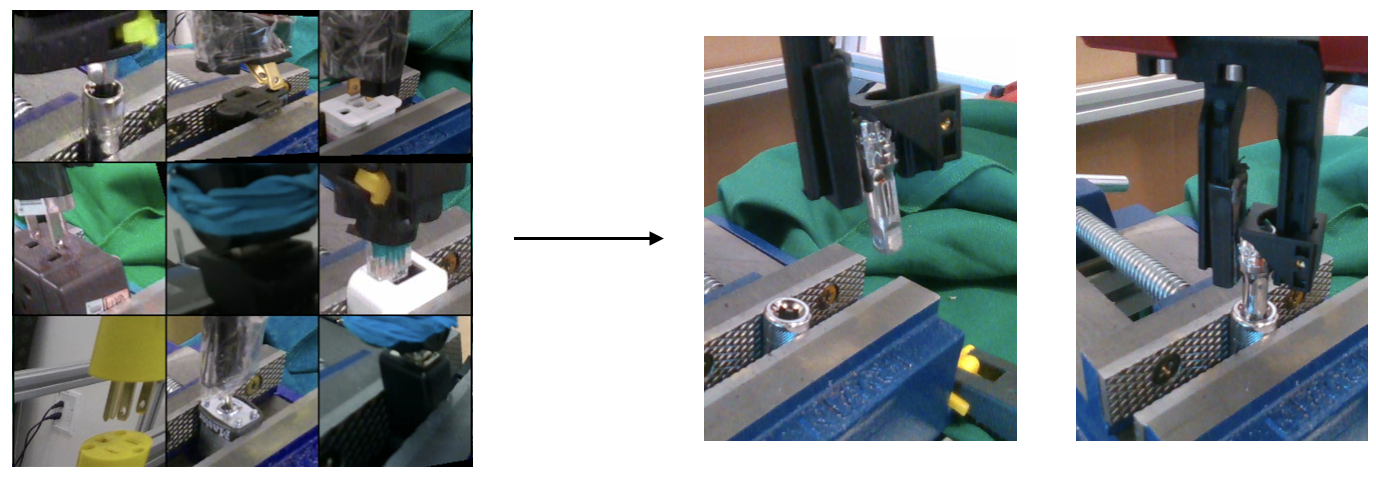
\includegraphics[width=0.7\textwidth]{imgs/fig1.png}
    \end{subfigure}

    \caption{We use offline reinforcement learning on insertion data on a diverse set of connectors (left) followed by online finetuning to solve a connector-socket insertion task from vision on a previously unseen connector (right).}
%%SL.6.8: Great to have a page 1 figure like this, but it would be good if it actually provides a diagram illustrating the method at a high level, rather than just some robot pictures (though it's good of course to show lots of connectors). I also found the photos to be extremely hard to parse. It's good that they're diverse, but I can barely see the connector in most of them.
    \label{fig:novel_obj}
    \vspace{-0.5cm}
% \end{wrapfigure}
\end{figure}

% Our solution
% {
% \color{blue}
% (Proposed fix, haven't seen gains from this yet.)
% }
% We propose to use an auxiliary contrastive representation learning objective that aligns disparate domains to address this issue.
% %%SL.5.25: not quite clear what "disparate domains" refers to here
% To learn low-dimensional representations from large (160x160) image input for sample-efficient RL, we use the standard self-contrastive learning objective with data augmentations.
% %%SL.5.25: that doesn't sound like a contribution, it kind of just sounds like we use a thing that already exists
% To align data from diverse domains, we additionally treat all observations with positive rewards (i.e., images of successful insertions) as positives.
% During online finetuning, this auxiliary objective can be used in combination with online RL with a high number of gradient updates per environment step to stabilize and accelerate learning.

% % Contributions
% We present three key contributions.
% First, a novel representation learning method that enables fast finetuning of vision-based IQL policies on a new domain. 
% %%SL.5.25: this is not a complete sentence! also, you said before it's a standard method, but now it's a novel method?
% Second, a system based off of this representation learning method to insert robustly from vision without the need of state information, both for observations and rewards.
% We show that new tasks can be learned within X trials, given our dataset of off-policy data from Y prior tasks of Z trajectories.
% This system allows us to finetune a connector with grasping in the loop {\color{blue}
% (assuming this works.)}.
% Using this system, we collected high-quality insertion data on Y connectors.
% %%SL.5.25: why is this important?
% Our third contribution is to release a dataset for robotic insertion connectors, as well as pretrained features and reward models.
% %%SL.5.25: this kind of comes out of nowhere, wasn't mentioned or discussed before; if the dataset is one of the contributions, you would need to actually discuss it in detail and explain how it's useful to people (you could just remark that we release the dataset without claiming that it is one of the contributions, if you don't want to deal with this problem)
% Our dataset will be made public at <URL>.

\section{Related Work}

%%SL.6.2: Remember that the organization of the related work should reflect the contribution of the paper. It makes sense to start by talking about reinforcement learning for robotics if we position the paper such that this is the core area of the paper. But right now the intro positions the paper first and foremost as a contribution in industrial insertion, making this rather incongruent.

Our work proposes a novel representation learning method for reinforcement learning to enable successful finetuning on a test domain after offline RL on a dataset with few domains. This method is applied to real-world robotic insertion problems. In this section, we discuss prior work on representation learning, reinforcement learning for robotics, and industrial insertion.
%%SL.6.8: could probably cut the above para if we're short on space or replace with one sentence; you could also cut the paragraph headings and start the first para with a transition sentence (in fact the sentence is already a good transition...)

\textbf{Representation learning objectives for reinforcement learning.}
Many prior methods have explored representation methods for improving the sample efficiency of RL algorithms. These include reconstructive objectives \cite{lange2010deep, lange2012autonomous, finn2016deep}, bisimulation~\cite{ferns2004bisimulation, castro20bisimulation, zhang2021dbc}, and other auxiliary tasks \cite{jonschkowski2017pve, ghosh2018learning, sax2018midlevel}. 
Variational information bottleneck 
In this work, we expand on contrastive methods, which have been shown to provide good features for fine-tuning in many vision tasks [] and have also shown promise in RL~\cite{laskin2020curl}. 
%%SL.6.8: lots of other contrastive methods in RL besides this... (e.g., nearly all non-reconstructive MBRL methods)
% Another related class of methods is bisimulation~\cite{ferns2004bisimulation, castro20bisimulation, zhang2021dbc}, which attempts to learn task-specific features via learning a bisimulation metric.
We use contrastive learning but differ from prior work in two important ways.
First, we use contrastive learning for the purpose of aligning offline data, where we have curated rewards and near-optimal data, with online reinforcement learning data that might be arbitrarily poor.
Second, we align domains with the contrastive learning objective in our application domain by aligning all states with positive reward.
%%SL.6.8: repetitive use of "align" and "domain" above (but otherwise reads well!)

Closely related to our work is work on domain adaptation. Domain adaptation methods generalize from source domains to a target domain, usually by matching the distribution of features between domains via matching statistics~\cite{tzeng2014domainconfusion, sun2016coral, long2015adaptation} or using an adversarial loss~\cite{ganin2016domainadversarial, Bousmalis2016}.
Successfully matching distributions makes features indistinguishable; however, in our case, it may be possible that domain-specific information is also important.
In robotics, domain adaptation has been applied successfully in the sim-to-real setting~\cite{bousmalis2017simtoreal, james218simtosim}.

In this work, we focus on two unique aspects of representation learning for reinforcement learning. First, stabilizing and accelerating finetuning of convolutional neural network policies. Second, aligning domains via reward labels in order to generalize well to new domains and finetune quickly in the new domain.
%%SL.6.2: ok, but this paper is not the first to do either of those things, so what's the difference? are there more relevant prior works to contrast to? DA methods?
%%SL.5.25: In general, I think the representation learning version of the story will require very extensive discussion of how the proposed method is different from the *many* prior representation learning methods, and probably quite a few comparisons to the most relevant ones
%%AVN.6.2 My idea was that the representation learning part of the story is targeted to a pretty specific need - generalizing between different connectors, and finetuning. In this sense it is fine if the proposed thing is similar to something that exists (eg. contrastive), if the proposed modification does better on these two criteria. I guess the missing thing here though is transfer learning
%%SL.6.2: related work still needs to discuss the differences, above is not an excuse to just skip over most prior work in this area


\textbf{Reinforcement learning for robotics.}
% Model-free deep reinforcement learning algorithms in particular have shown human-level or superhuman performance using rich observations on sequential decision making tasks such as games~\cite{mnih2013atari, silver2016alphago}.
%%SL.5.25: what does this have to do with the previous sentence about robotics tasks?
%%AVN.6.2. reordered, to make the point that model-free RL for robotics is a good idea if done offline
%%SL.6.2: It still doesn't make sense to me -- why start a paragraph on RL for robotics with a sentence about RL that has nothing to do with robotics? It might kind of make sense if the sentence was about foundational work in RL, but that's not what is cited either.
% However, these algorithms have usually been trained from scratch,
%%SL.6.2: nitpick -- it's not the algorithms that are trained, it's policies that are trained via those algorithms
% which can be prohibitive for real-world robotics.
%%SL.6.2: there are plenty of papers on training robotic policies with RL from scratch, so obviously it is not prohibitive (and authors of those papers are likely to be reviewing this paper, and will reject it for deceptive discussion of related work)
Reinforcement learning has been applied successfully to a variety of robotics tasks in both manipulation~\cite{peters2008baseball, kober2008mp,deisenroth2011pilco, levine2016gps, levine2017grasping} and locomotion~\cite{giusti15trails, nakanishi2004bipedlfd, kalakrishnan09terraintemplates} settings.
%%SL.6.2: not sure what the significance of "model-based control" here is (and most of those papers don't use it, unless you consider PD control "model-based", which it isn't)
To utilize offline datasets with diverse data, specialized algorithms have been developed~\cite{chebotar2021actionable, kalashnikov2021mtopt, nair2020awac}.
%%SL.5.25: need to explain the difference (there are many works on offline pretraining now)
In this work, we focus on applying offline RL and fine-tuning from vision in the industrial insertion setting.
This setting poses unique challenges due to the need to generalize from few domains, which we address via representation learning.
%%SL.6.2: This is a really weak paragraph for related work. Can you discuss the most closely related stuff and explain how this paper is different? The above paragraph says more or less nothing about the distinction between the prior work and this paper.
%%AVN.6.8: if representation learning is the main thing, is there a need to communicate a distinction between this and prior RL papers (without represnetation learning) if it is covered in the previous paragraph?

\textbf{Robotic insertion.}

Prior work has discussed reinforcement learning for robotic insertion.
Initial work in this direction focuses on learning
%%SL.6.2: initial work in this direction has nothing to do with learning and is much older than this
for a single connector from ground-truth state information~\cite{lian2021insertionbenchmark, johannink18residualrl, schoettler2019insertion}.
In this case, the RL algorithm must learn to navigate the specific dynamics of the single connector, but does not generalize across connectors.
More recent work has considered using meta-learning to generalize and improve few-shot between domains~\cite{Schoettler2020}.
Zhao et al.
%%SL.6.2: citation?
use offline reinforcement learning and finetuning combined with  meta-learning to adapt to a new connector.
This work assumes a known position of the socket and consistent grasping of the connector, and is robust to a small amount ($\pm1mm$) of noise.
In this regime, the learning algorithm must learn a structured noise or exploration strategy that can overcome these errors.
%%SL.6.2: a bit ambiguous if "this regime" refers to this paper or prior paper
In contrast, we initialize connectors within $\pm2cm$ of the socket (20$\times$ the initial variance), which requires the robot to rely on visual feedback.

Closest to our work is prior work that also uses pixel input for robotic insertion.
Luo et al. incorporate vision alongside proprioception, using a VAE to embed pixel input~\cite{luo2021insertion}.
InsertionNet uses a vision system to localize the object and socket, operating on a "residual policy" which is learned from state by supervised learning~\cite{spector2021insertionnet}.
InsertionNet 2.0 incorporates contrastive representation learning to improve performance.
Distinct from these works, our method does not require any state information, which also makes it robust to significantly larger variation in initial connector pose.
%%SL.5.25: I think it will be hard to sell "doesn't require arm position" as a notable strength to a robotics audience (it's always there, why not use it?)
%%AVN.6.2: not arm position but rather localization of the socket and/or connector grasp. Hopefully the changes in the intro have addressed this better
%%SL.6.2: need to state this explicitly then -- but insertionnet doesn't require known position of the socket, does it?

\section{Background}

\subsection{Reinforcement learning.}

\subsection{Offline reinforcement learning and fine-tuning.}


\subsection{Representation learning.}

\section{Method}

The overall goal of our method is to be able to learn to insert previously unseen connectors. Because this requires domain generalization, we will first describe our representation learning objective that enables this. We will then describe how we train reward functions that generalize to new domains using this objective. Finally, we will describe the offline RL and online fine-tuning method with this representation that allows us to generalize policies and value functions to new scenes.

\subsection{Information constrained domain generalization.}

For some data $X$ with domain label $D$ and objective $L(f_\theta(X))$, we wish to minimize $L(f_\theta(Z))$, with the representation $Z=g_\phi(X)$, on an unseen domain by generalizing from few domains. However, full domain invariance is not what we want. If our representation was completely domain invariant, it could not take advantage of the domain-specific information about certain connectors: when the reward is obtained for each connector visually, domain-specific cues that the policy or Q function can take advantage of, and so on.

Instead, we can consider a split representation $Z = (Z_I, Z_S)$ consisting of a domain invariant representation $Z_I$ and a domain specific representation $Z_S$. We optimize

$\mathcal{L(Z)} - I(Z_I; D) \text{s.t.} I(X; Z) \leq C$.

Following~\citet{alemi2017vib}, this becomes

$\min_{\theta, \phi} \mathcal{L(Z)} - I(Z_I; D) - \beta I(X; Z)$.

We optimize the $I(Z_I; D)$ term using domain adversarial networks and $\beta I(X; Z)$ using a variational information bottleneck.

\subsection{Reward learning and labeling.}

Next, we will describe how we incorporate domain generalization for learning a reward function that generalizes.

\subsection{Offline reinforcement learning.}

Next, we will describe how we incorporate domain generalization into IQL.

\subsection{Online finetuning}

Next we will describe the online finetuning procedure

\section{Experiments}

We design our experiments to answer the following questions.
\begin{itemize}
    \item Does representation learning improve accuracy for reward classification?
    \item Does offline reinforcement learning followed by online fine-tuning outperform baselines?
    \item Does vision-based RL outperform state-based methods in the presence of noise?
    \item Is offline reinforcement required (as opposed to behavior cloning)?
    \item What is the model paying attention to?
    \item Can the learned features transfer to a new robot?
\end{itemize}

\subsection{Reward Classification}

To evaluate the proposed method 
We present results on the reward classifier, evaluated on a set of five held-out connectors: .

VIB + DAN: 88\% accuracy 

DAN only: 71\% accuracy

DAN + extra (VIB weight=0): 77\% accuracy

VIB only: 79\%

no representation: 76\% accuracy

\subsection{Self-Supervised Fine-tuning}

Does it finetune?

We compare against the following baselines:
- localization

\subsection{Effect of Vision}

Better than state-based training? - with this amount of variation, it definitely is

\subsection{Reinforcement Learning vs IQL}

Is offline RL better than BC?

Could show some value function

Better than basic representation learning methods? Eg. contrastive / ImageNet pretraining / reconstructive

\subsection{Inspecting the Networks}

Inspecting the learned features - does it focus on edges to line up in a scene, etc.?

\subsection{Generalizable Reward Functions}

Can the learned features transfer to a new robot? (evaluate reward prediction accuracy)

\begin{figure}[t]
    \centering
    \begin{subfigure}[b]{0.99\linewidth}
        \center
        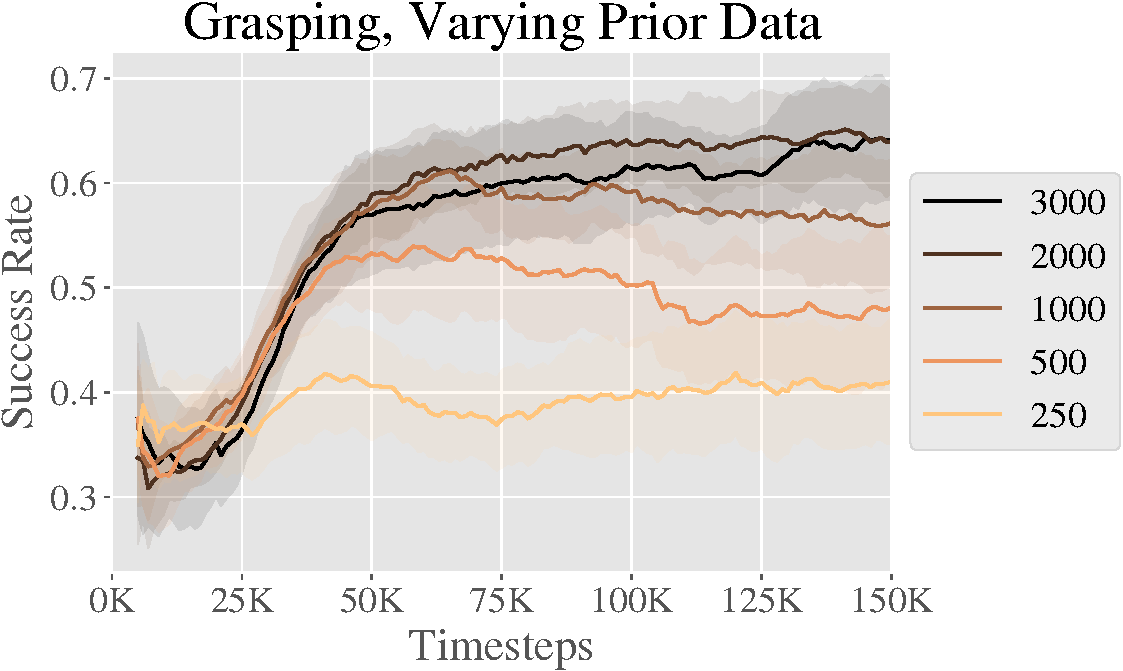
\includegraphics[width=0.6\textwidth]{imgs/vary_data-crop.pdf}
    \end{subfigure}

    \caption{[PLACEHOLDER FROM PREVIOUS WORK - VAL] Learning curves for simulated grasping of novel objects with VAL, using data from an increasing number of training objects for offline RL. We collect 50 trajectories per training object, and each line is labeled with the total number of training trajectories. \textit{We want to show something similar on real-world connectors.} }

    \label{fig:novel_obj}
    \vspace{-0.5cm}
% \end{wrapfigure}
\end{figure}

\section{Results}

\section{Discussion}


%===============================================================================

% no \bibliographystyle is required, since the corl style is automatically used.
\bibliography{example}  % .bib

\end{document}
